\section{Limit plots}

The PoI for the scans is the signal strength $\mu = \sigma / \sigma_{SM}$, and the ggF and VBF channels are fit simultaneously.
The results for the \kl scan and \kvv scan are shown in \Fig{\ref{fig:comb_kl_scan}} and \Fig{\ref{fig:k2v-comb}}, respectively.

\begin{figure}[h]
	%\centering
	\subfloat[\kl scan]{
		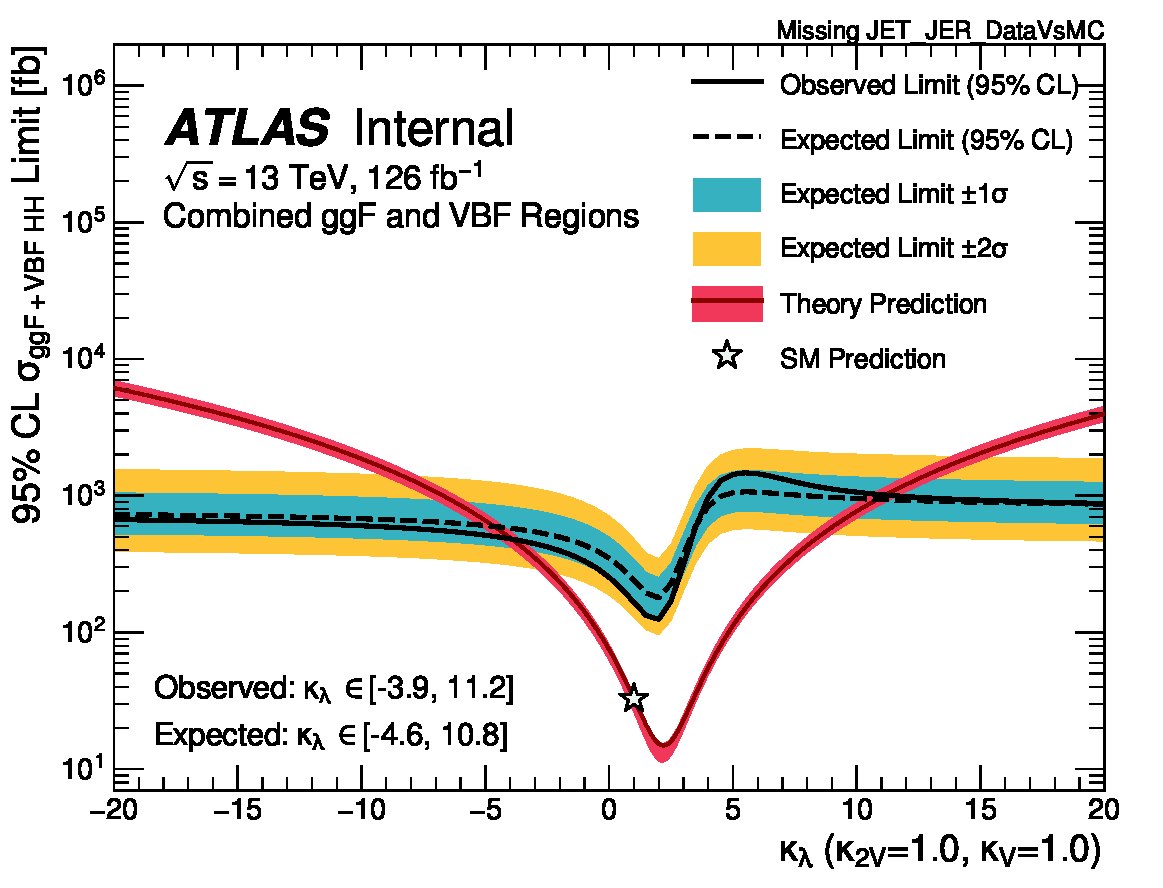
\includegraphics[width=0.45\textwidth]{\figDir/kl_scan_correlated_fullsyst_unblind_ggF_VBF_comb_samps_ggf_and_vbf_pd_ggf_161718_vbf_inc161718_k2v_1.0_xs.pdf}
		\label{fig:comb_kl_scan}
	}
	\subfloat[\kvv scan]{
		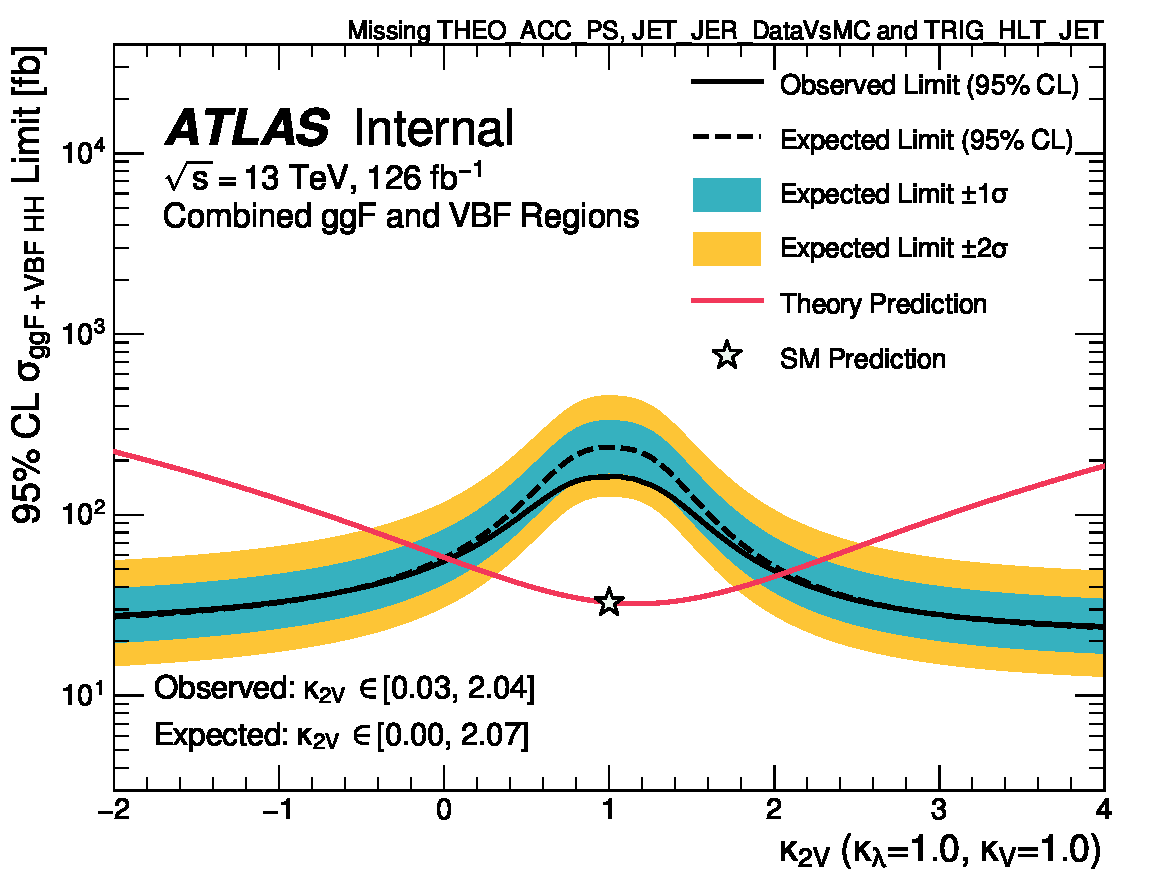
\includegraphics[width=0.45\textwidth]{\figDir/k2v_scan_correlated_fullsyst_unblind_ggF_VBF_comb_k2v_samps_ggf_and_vbf_pd_ggf_161718_vbf_inc161718_kl_1.0_xs.pdf}
		\label{fig:k2v-comb}
	}
	\caption{The 95\% CLs limit on the combined ggF and VBF \HH production cross-sections with respect to the \kl variations (left) and the \kvv variations (right).}
	\label{fig:comb-scans}
\end{figure}

The limit on the SM signal strength is 5.4 (8.1) observed (exp). 
To understand which systematics are driving our performance, a couple of other expected upper limits are calculated.
The limit with only the statistical uncertainties included (the 2b stat uncertainty and signal mc stat uncertainty), our limit would have been 6.0. The limit just including the background systematic uncertainties is 7.1. Furthermore, \Tab{\ref{tab:systematics}} shows the impact of the dominant systematics on our SM limit. The dominant systematic from the experimentalist side come from the background systematics, with the NN retraining errorbar and the systematic quantifying our extrapolation into the SR being of roughly equal size and having a 7\% impact on our final result. The current uncertainty on the theoretical HH cross-section has a 9\% impact on our result. 
%%%%%%%%%%%%%%%%%%%%
% Systematics breakdown table
%%%%%%%%%%%%%%%%%%%%
\begin{table}%[!tbh]
	\centering
	\begin{tabular}{l r}
	\toprule
		   Source of uncertainty \qquad & $ \Delta \mu / \mu$ \\
             \hline
             \textbf{Theoretial}                                        &   \\
                         Uncertainty on signal cross-setion               & $-9.0$\%  \\
                         All other theory uncertainties                        & $-1.4$\%  \\
              \hline
              \textbf{Background modeling }                                &   \\
                         NN retraining + bootstrap                             &  $-7.1$\%  \\
                         CR1 / CR2 extrapolation                              &  $-7.5$\%  \\
                         3b1f non-closure uncertainty                       &  $-2.0$\%  \\
              \bottomrule

	\end{tabular}	
\caption{Impact of the various uncertainties on the $\mu_{ggF+VBF}$ limit.
To test the impact of each systematic, it's profiled and then constrained to its best fit value as the upper limit is recalculated.
Only the systematics that have an impact larger than a \% are shown. 
Note -- all of the experimental uncertainties together had a sub-\% level impact on the final result.}
\label{tab:systematics}
\end{table}

The observed (expected) upper limit on the SM ggF+VBF signal strength, including the cross section uncertainty from theory calculations, is 5.45 (8.09) and shown in Table \ref{table:ggfvbf-sm-xs-tab}. The limit set on \kl using the combined ggF and VBF channels are the strongest constraints set on this coupling in the \bbbb final state in ATLAS to date. 

Expected and observed upper limits on the ggF+VBF cross section are $7.36 \times 32.776 = 241.20$ $5.02 \times 32.776 = 164.49$, where the theory calculation uncertainties on the ggF and VBF cross sections are excluded.

\begin{table}
	\centering
	\begin{tabular}{c c c c c c c}
		\toprule
		{} & {Observed} & {$-2\sigma$} & {$-1\sigma$} & {Expected} & {$+1\sigma$} & {$+2\sigma$}\\
		\midrule
		{ggF production: ggF channel fit} & {5.73}  & {4.44} & {5.97} & {8.28} & {12.51} & {19.71}  \\
		{ggF production: ggF+VBF channels fit} & {5.51}  & {4.41} & {5.92} & {8.22} & {12.43} & {19.62}  \\
		{VBF production: VBF channel fit} & {122.9}  & {72.0} & {96.7} & {134.3} & {194.2} & {281.6}  \\
		{VBF production: ggF+VBF channels fit} & {132.3}  & {71.3} & {95.7} & {132.8} & {191.9} & {277.7}  \\
		{ggF+VBF production: VBF+ggF channels fit} & {5.45} & {4.34} & {5.83} & {8.09} & {12.21} & {19.19} \\
		\bottomrule
	\end{tabular}
	\caption{The observed and expected upper limit on the SM \HH production cross-section at the 95\% CL. The expected value is shown with corresponding one and two standard deviation error bounds.}
\label{table:ggfvbf-sm-xs-tab}
\end{table}


\kl values where the limit set on the cross-section is below the theoretical value are excluded at the 95\% CL. The constraint set on \kl from the combination of the ggF and VBF channels is shown in Table \ref{table:kl-chan-comp-tab} alongside the constraints from the individual channels.



\begin{table}[h]
	\centering
	\begin{tabular}{c c c}
		\toprule
		{Channel} & {Observed Interval} & {Expected Interval} \\
		\midrule
		{ggF Channel (ggF signal only)} & {$[-4.5, 13.3]$} & {$[-5.0, 12.0]$}  \\
		{VBF Channel (VBF signal only)}  & {$[-10.0, 13.2]$} & {$[-12.3, 15.6]$} \\
		{Combination (ggF+VBF signals)} & {$[-3.9, 11.2]$} & {$[-4.6, 10.8]$}  \\
		\bottomrule
	\end{tabular}
	\caption{In the combined channel, the observed and expected limit intervals on the coupling modifier \kl at the 95\% CL for the ggF channel, the VBF channel and the combination of the two.}
\label{table:kl-chan-comp-tab}
\end{table}


%%%%%%%%%%%%%%%%%%%%
% 2d limit
%%%%%%%%%%%%%%%%%%%%

The 2D limit on the \kvv and \kl variations for the combined ggF + VBF channels is shown in \Fig{\ref{fig:2d-lim}} assuming \kv = 1.
Limits are derived from the intersection of the cross-section limit and the theory predictions at given point.

\begin{figure}[ht]
	\centering
	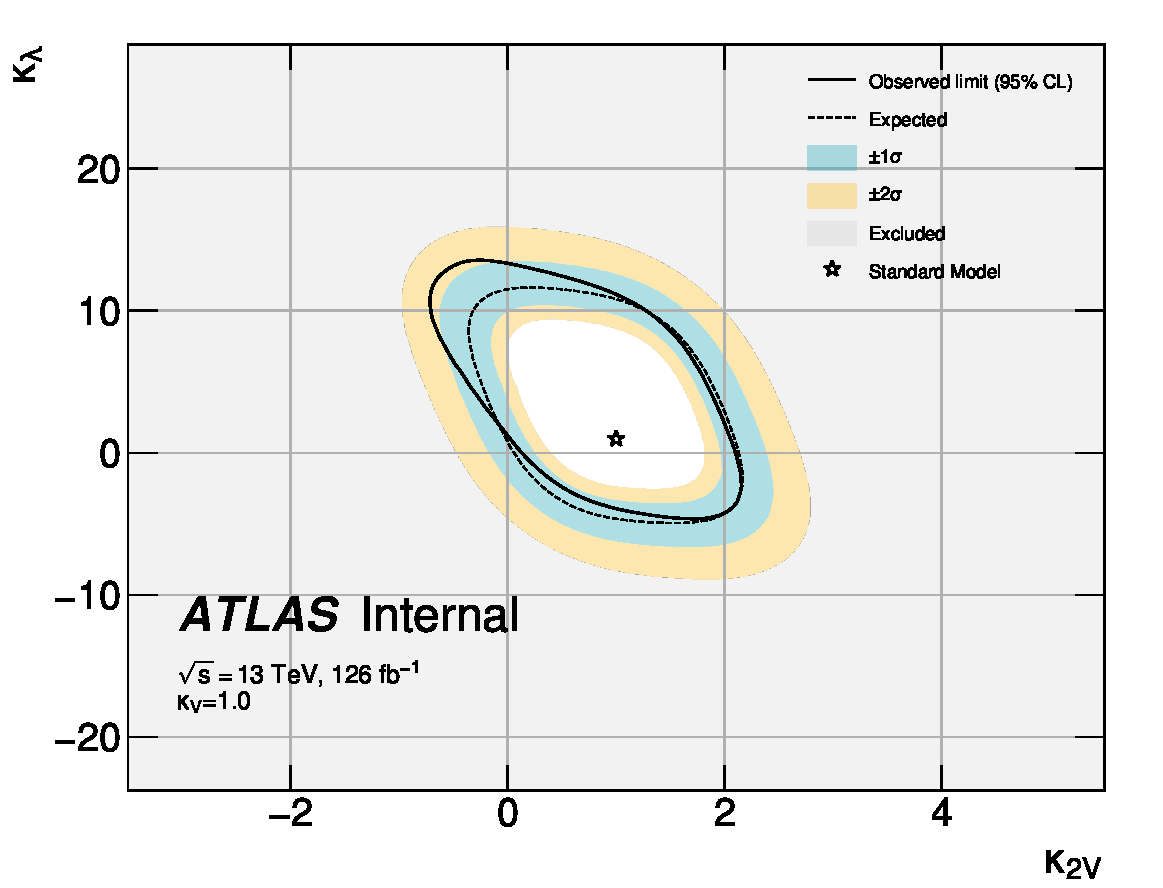
\includegraphics[width=0.44\textwidth]{\figDir/2D_scan_ggF_VBF_comb_samps_ggf_and_vbf_pd_ggf_161718_vbf_inc161718_k1v1.0_exclusion.pdf}
	\caption{The obs (solid) and expected (dashed) limit intervals on the coupling modifiers \kl vs \kvv  at the 95\% CL for the combination of the VBF+ggF channels.}
	\label{fig:2d-lim}
\end{figure}

\subsection{Improvements from previous analyses}

\textbf{To do: Make the history of the analysis plot!!}

\textbf{To do: Remake the cat improvements plots!!}

% To demonstrate the expected improved sensitivity from the addition of the \deta and \Xhh categories, a comparison of the SM signal limits with and without these categories is shown in \Fig{\ref{fig:sm-limit}} on the pre-fit Asimov dataset with background CR12 shape uncertainties only and with the decorrelated scheme.
% The categorization gives us a $\sim$30\% improvement in the SM limits. 
% \Fig{\ref{fig:kl-scan-ratio}} shows the corresponding \kl scan and the corresponding increase in sensitivity from the categorization.\footnote{For these limits, finer \mhh binning in the \mhh inclusive fit is used to maintain a similar number of bins with and without categorization.}

% \begin{figure}[ht]
% 	\centering
% 	\subfloat[]
% 	{
% 	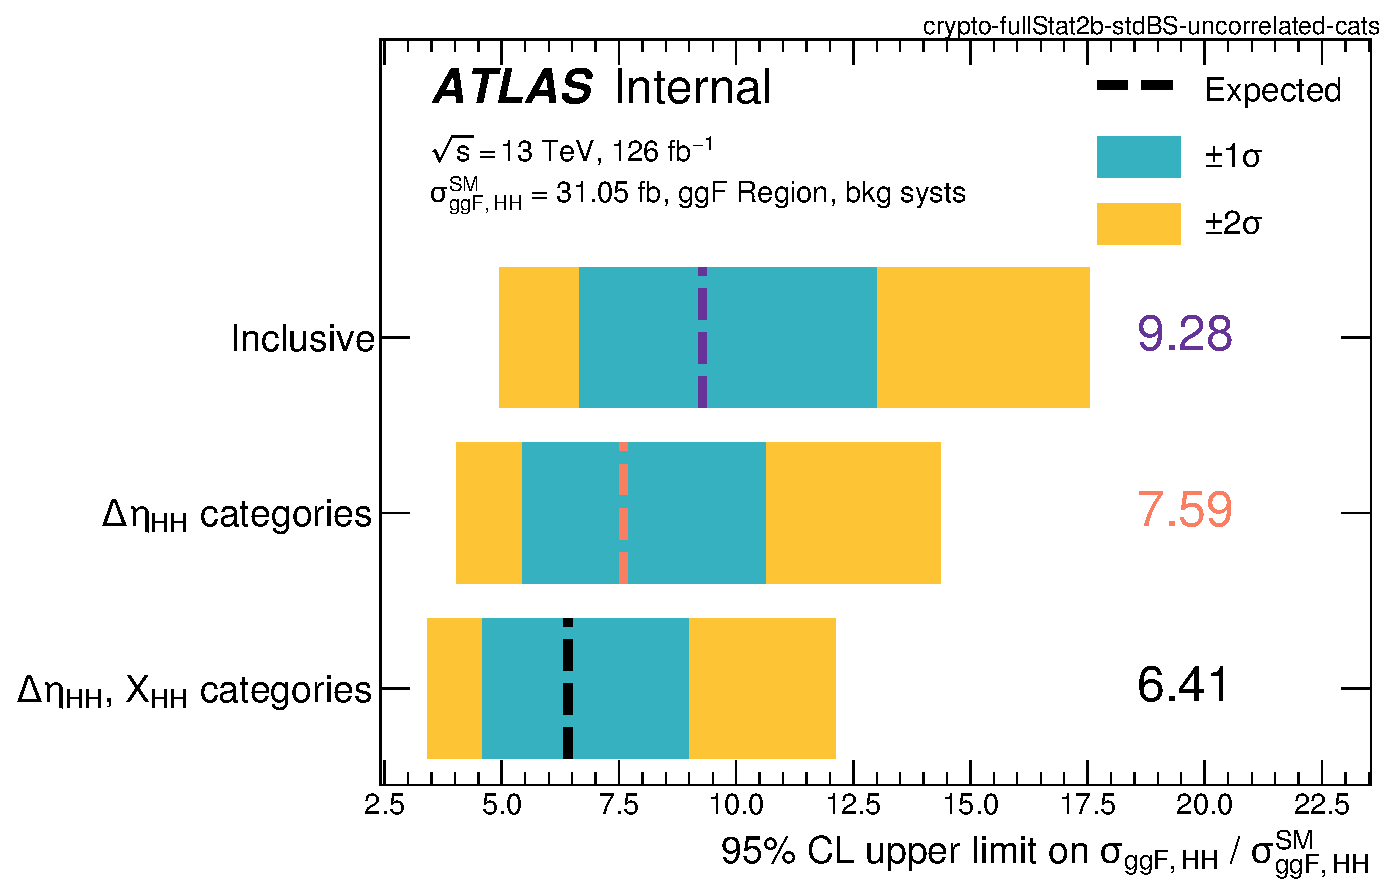
\includegraphics[width=0.44\textwidth]{sm-lim-uncorr}
% 	\label{fig:sm-limit}
% 	}
% 	\subfloat[]
% 	{
% 		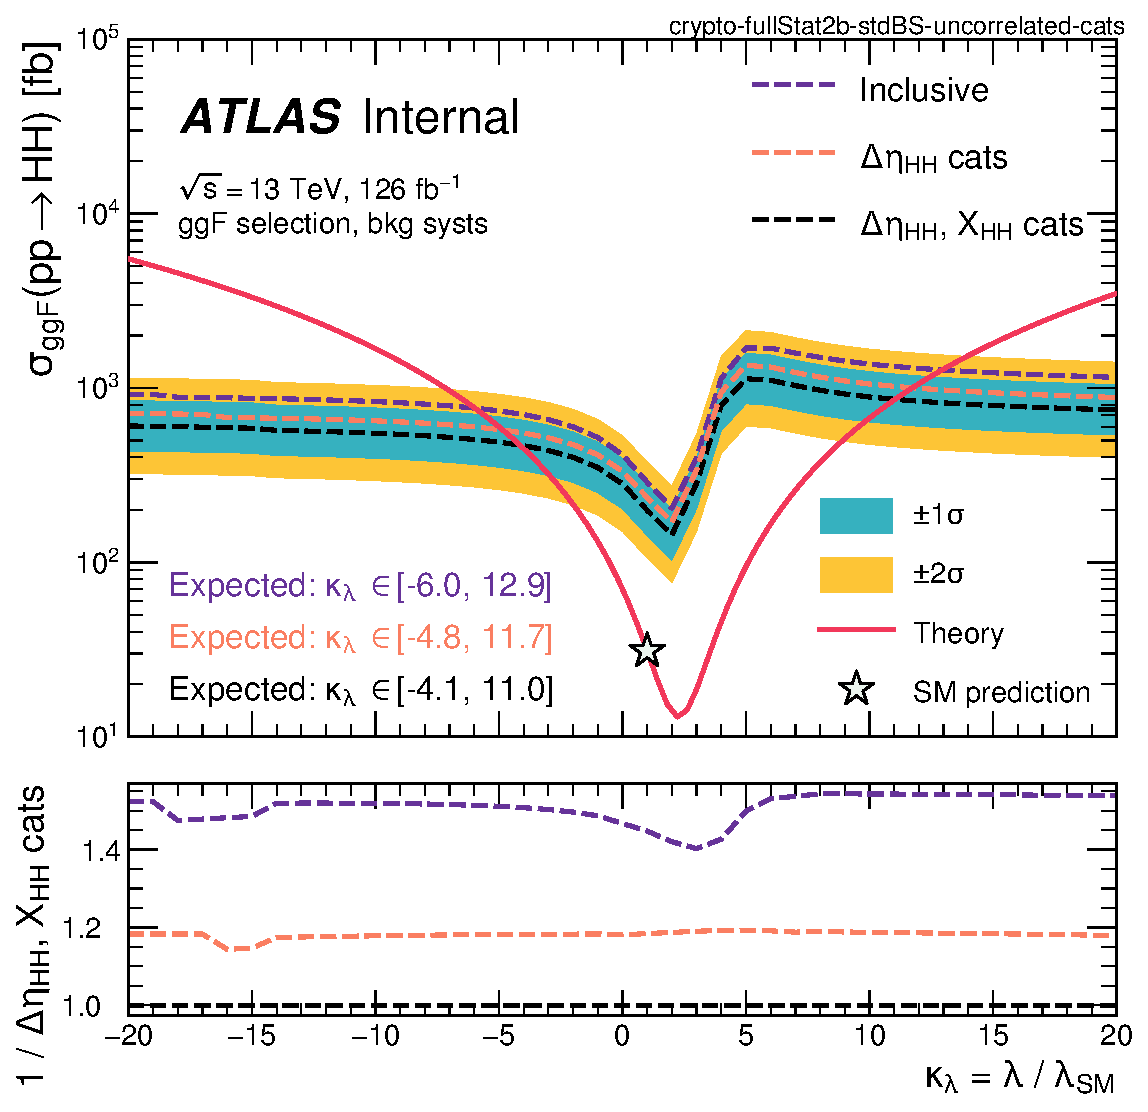
\includegraphics[width=0.5\textwidth]{kl-scan-uncorr-ratio-cats}
% 		\label{fig:kl-scan-ratio}
% 	}
% 	\caption{Expected sensitivity improvements for the ggF analysis by categorizing the fit discriminant (progressively adding \deta only, then the \Xhh categories).
% 	Studies are done on pre-fit Asimov with bkg-only systematics uncorrelated.
% 	 }
% 	\label{fig:ggF-ratio}
% \end{figure}




%%%%%%%%%%%%%%%%%%%%%%%%%%%%%%
% Other info
%%%%%%%%%%%%%%%%%%%%%%%%%%%%%%

% (1) The kl limit plot with the ggF chan and VBF chan constraints overlaid
%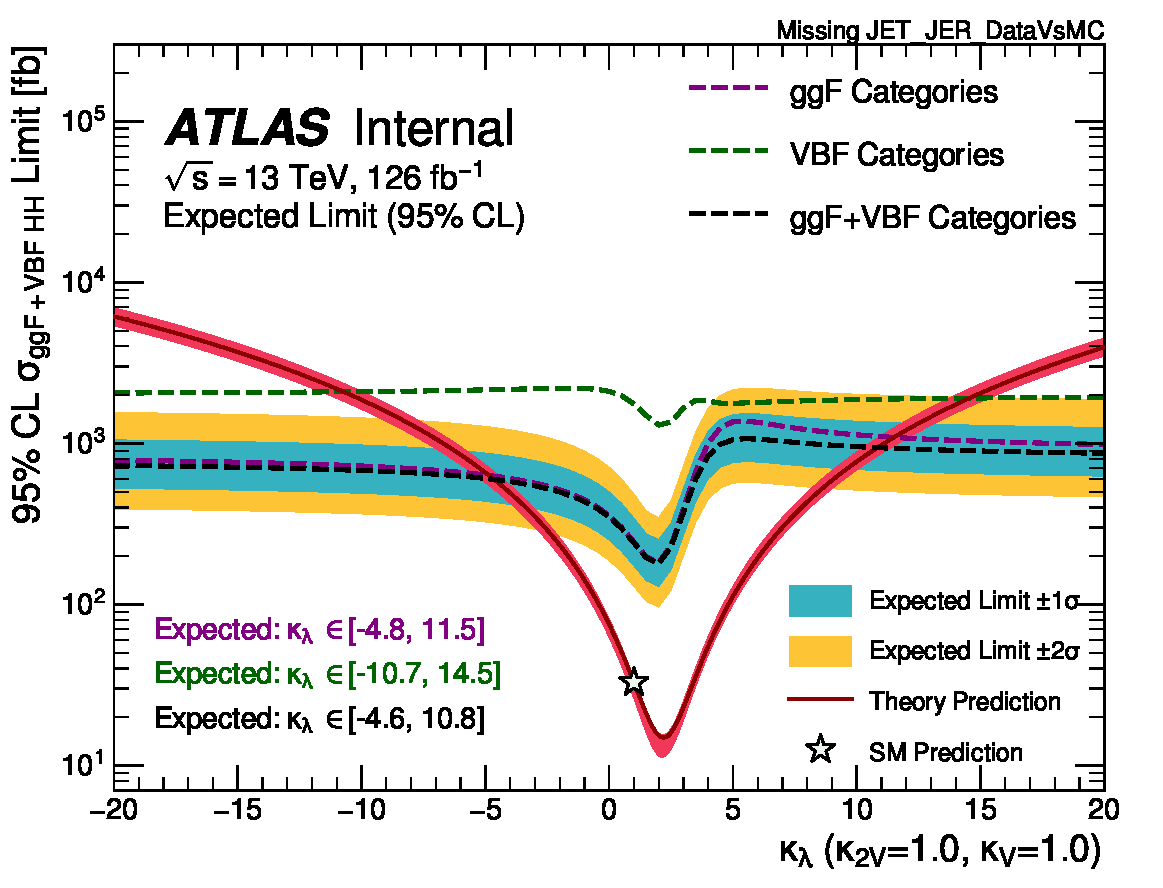
\includegraphics[width=0.45\textwidth]{\figDir/kl_scan_allcats_correlated_fullsyst_unblind_ggF_VBF_comb_samps_ggf_and_vbf_pd_ggf_161718_vbf_inc161718_k2v_1.0_xs.pdf} %{kl-scan-comb-uncorr-ratio-cats.pdf}

% (2) The k2v plot including just the VBF channel results
%The ggF production is accounted for as a (very sub-dominant) background process, and the limit is set on the VBF signal production.
% exp VBF chan constraint: k2v (-0.08,2.16)
% exp ggF+VBF chan const: k2v (-0.05, 2.12)
%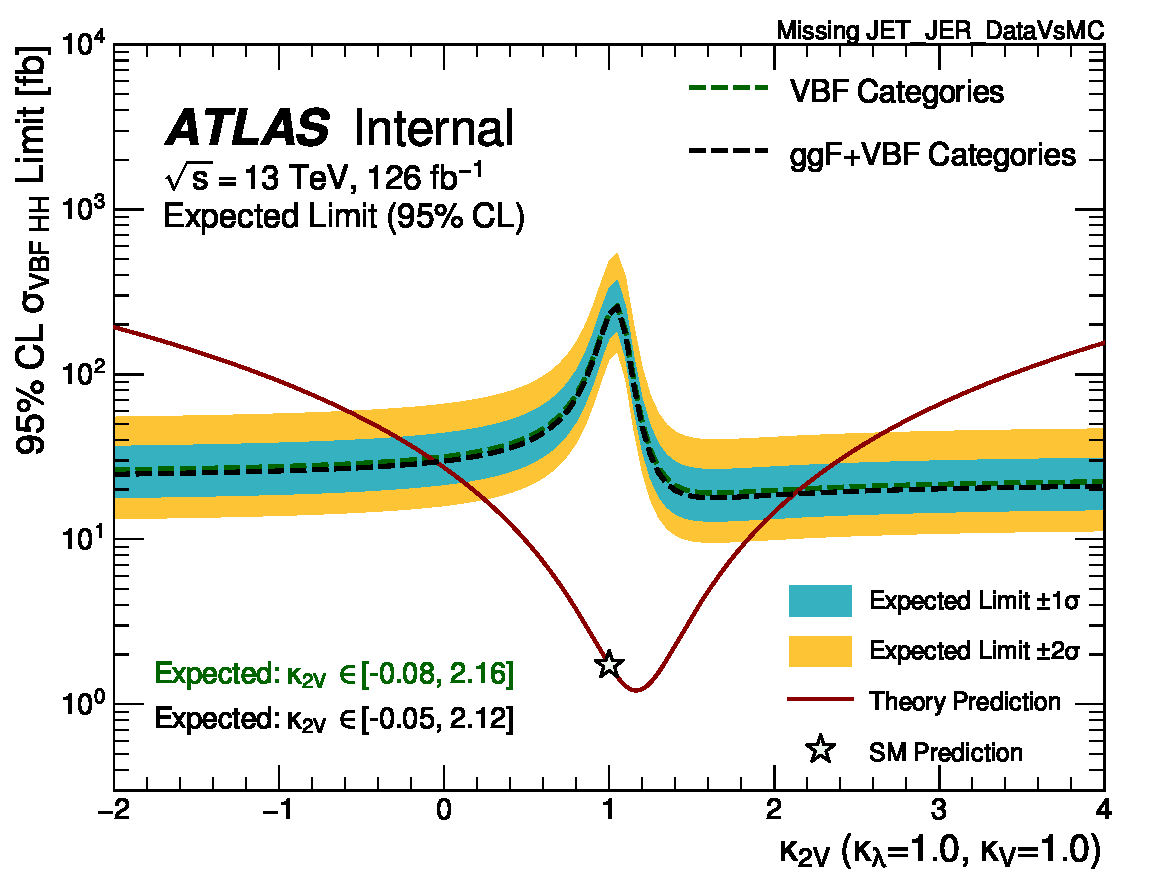
\includegraphics[width=0.45\textwidth]{\figDir/k2v_scan_allcats_correlated_fullsyst_unblind_ggF_VBF_comb_k2v_samps_ggf_and_vbf_pd_ggf_161718_vbf_inc161718_kl_1.0_xs.pdf}

% (3) k2v vs kv
% expected only, and the figure is pretty choppy
% 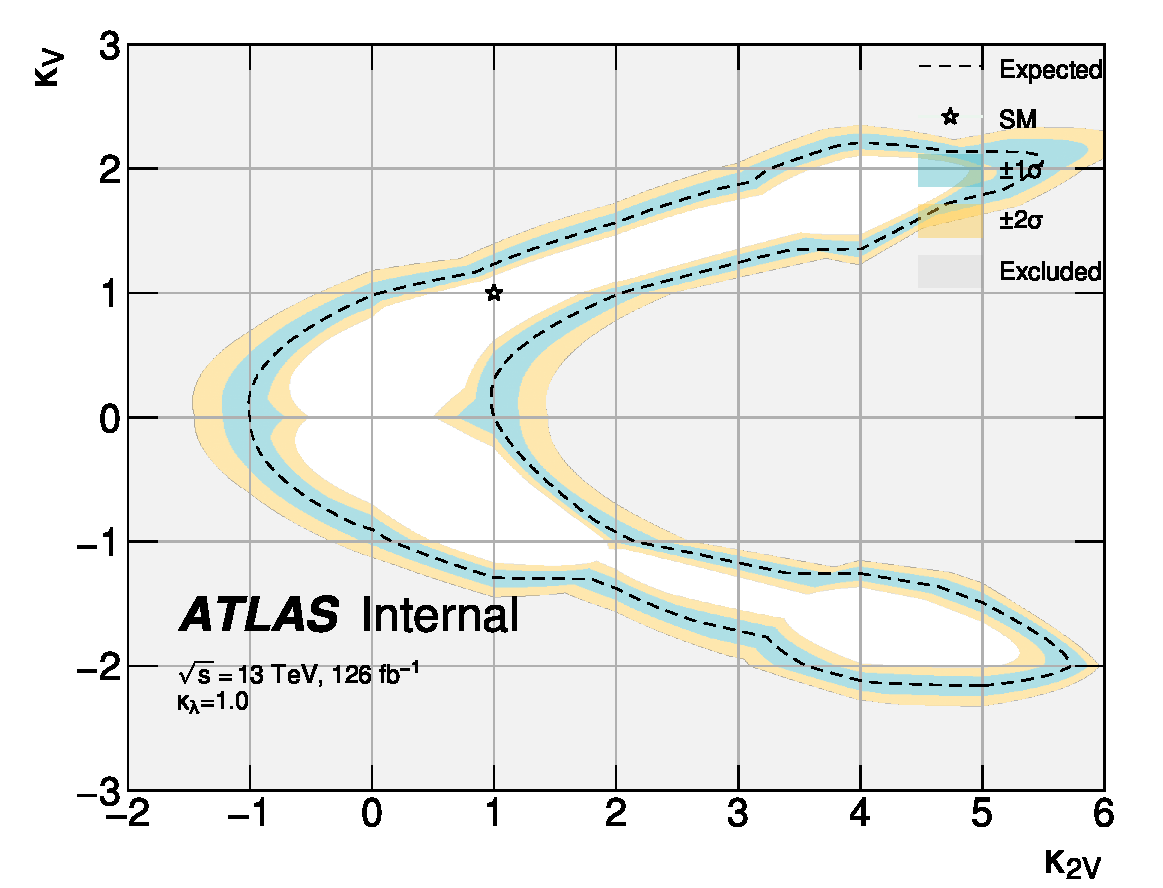
\includegraphics[width=0.44\textwidth]{figures/nr-int-note/results/V3/2D_scan_cmilke_full_3D_wide_scan_comb_samps_ggf_and_vbf_pd_ggf_161718_vbf_inc161718_kl1p0_exclusion.pdf}